\subsection{SGX Enclave Versioning Support}
\label{sec:sgx_versioning}

The software attestation model~(\S~\ref{sec:generic_software_attestation})
introduced by the Trusted Platform Module~(\S~\ref{sec:tpm}) relies on a
measurement~(\S~\ref{sec:sgx_measurement}), which is essentially a content
hash, to identify the software inside a container. The downside of using
content hashes for identity is that there is no relation between the identities
of containers that hold different versions of the same software.

In practice, systems based on secure containers need to handle software
updates, which entails having the ability to migrate secrets between the
container that has the old version of the software and the container that has
the updated version. This requirement translates into a need for a separate
identity system that can recogize the relationship between two versions of the
same software.

SGX supports the migration of secrets between enclaves that represent different
versions of the same software, as shown in
Figure~\ref{fig:sgx_secret_migration}.

\begin{figure}[hbt]
  \centering
  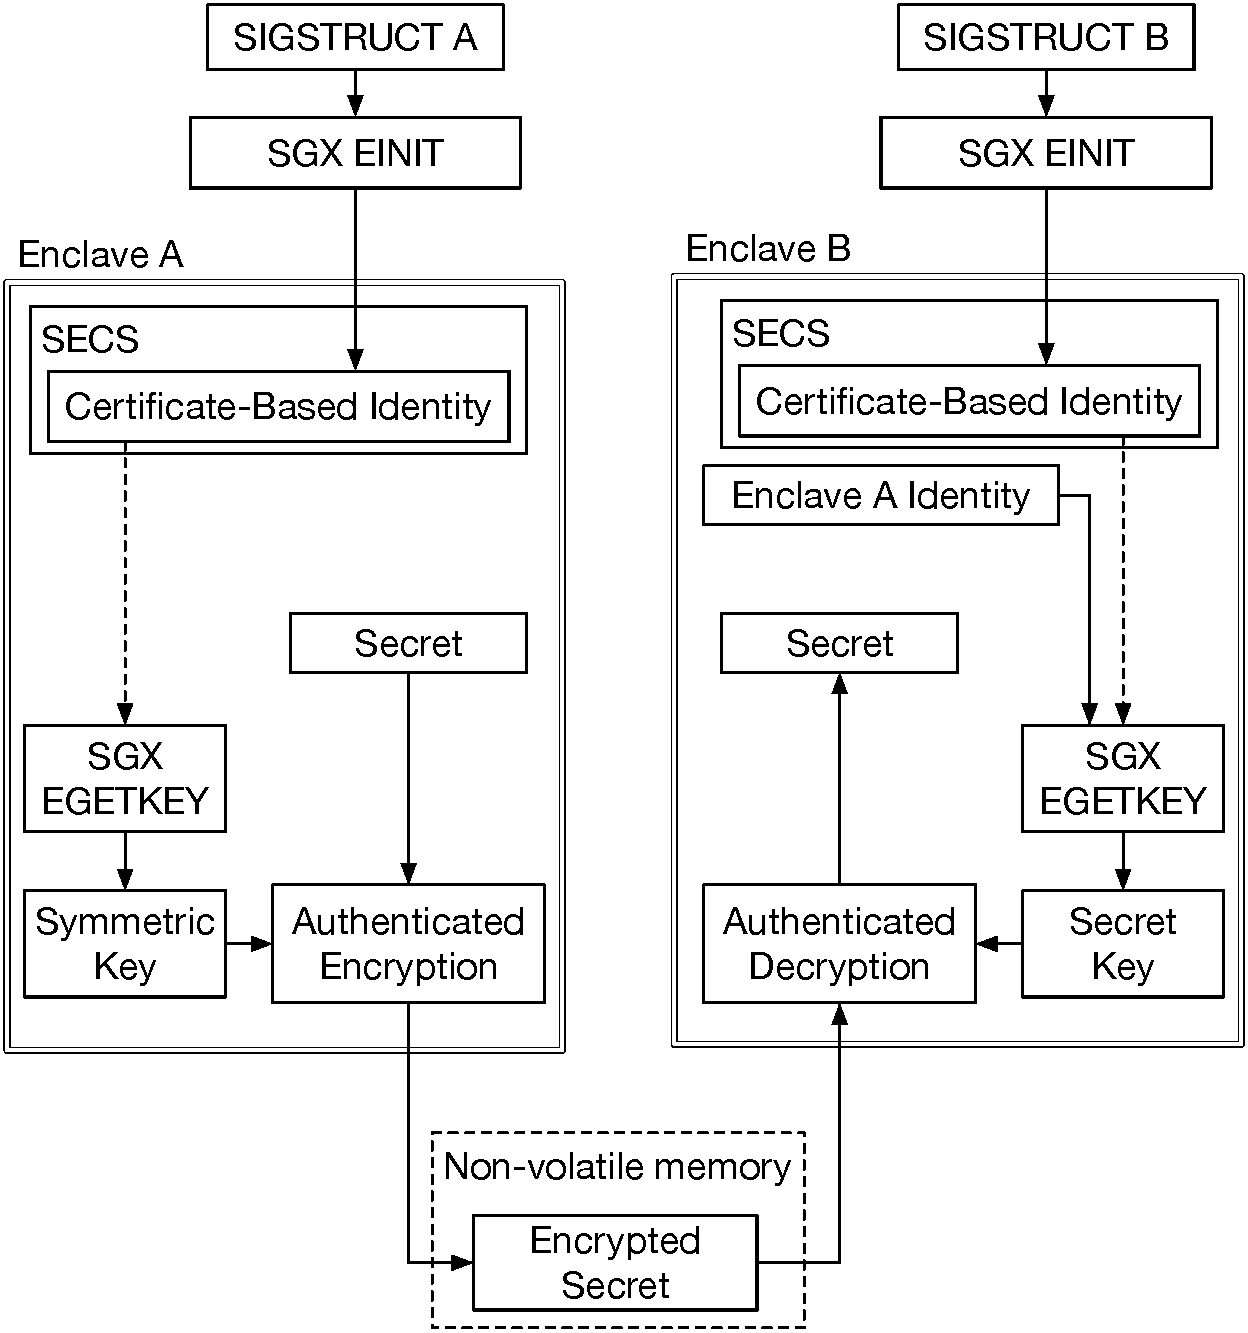
\includegraphics[width=87mm]{figures/sgx_secret_migration.pdf}
  \caption{
    SGX has a certificate-based enclave identity scheme, which can be used to
    migrate secrets between enclaves that contain different versions of the
    same software module. Here, enclave A's secrets are migrated to enclave B.
  }
  \label{fig:sgx_secret_migration}
\end{figure}

SGX's migration system relies on a one-level certificate
hierarchy~(~\S~\ref{sec:certificates}), where each enclave author is a
Certificate Authority, and each enclave receives a certificate from its author.
These certificates must be formatted as Signature Structures~(SIGSTRUCT), which
are described in \S~\ref{sec:sgx_sigstruct}. The information in these
certificates is the basis for an enclave identity scheme, presented in
\S~\ref{sec:sgx_certificate_identity}, which can recognize the relationship
between different versions of the same software.

The \texttt{EINIT} instruction~(\S~\ref{sec:sgx_einit_overview}) examines the
target enclave's certificate and uses the information in it to populate
the SECS~(\S~\ref{sec:sgx_secs}) fields that describe the enclave's
certificate-based identity. This process is summarized in
\S~\ref{sec:sgx_einit_sigstruct}.

Last, the actual secret migration process is based on the key derivation
service implemented by the \texttt{EGETKEY} instruction, which is described
in \S~\ref{sec:sgx_egetkey}. The sending enclave uses the \texttt{EGETKEY}
instruction to obtain a symmetric key based on its identity, encrypts its
secrets with the key, and hands off the encrypted secrets to the untrusted
system software. The receiving enclave passes the sending enclave's identity
to \texttt{EGETKEY}, obtains the same symmetric key as above, and uses the key
to decrypt the secrets received from system software.


\subsubsection{Enclave Certificates}
\label{sec:sgx_sigstruct}
\label{sec:sgx_mrsigner}

% Enclave Signature Structure (SIGSTRUCT): SDM S 38.13

The SGX design requires that each enclave must have a certificate issued by its
author. This requirement is enforced by
\texttt{EINIT}~(\S~\ref{sec:sgx_einit_overview}), which refuses to operate on
enclaves without valid certificates.

The SGX implementation consumes certificates formatted as
\textit{Signature Structures}~(SIGSTRUCT), which are intended to be generated
by an enclave building toolchain, as shown in Figure~\ref{fig:sgx_sigstruct}.

\begin{figure}[hbt]
  \centering
  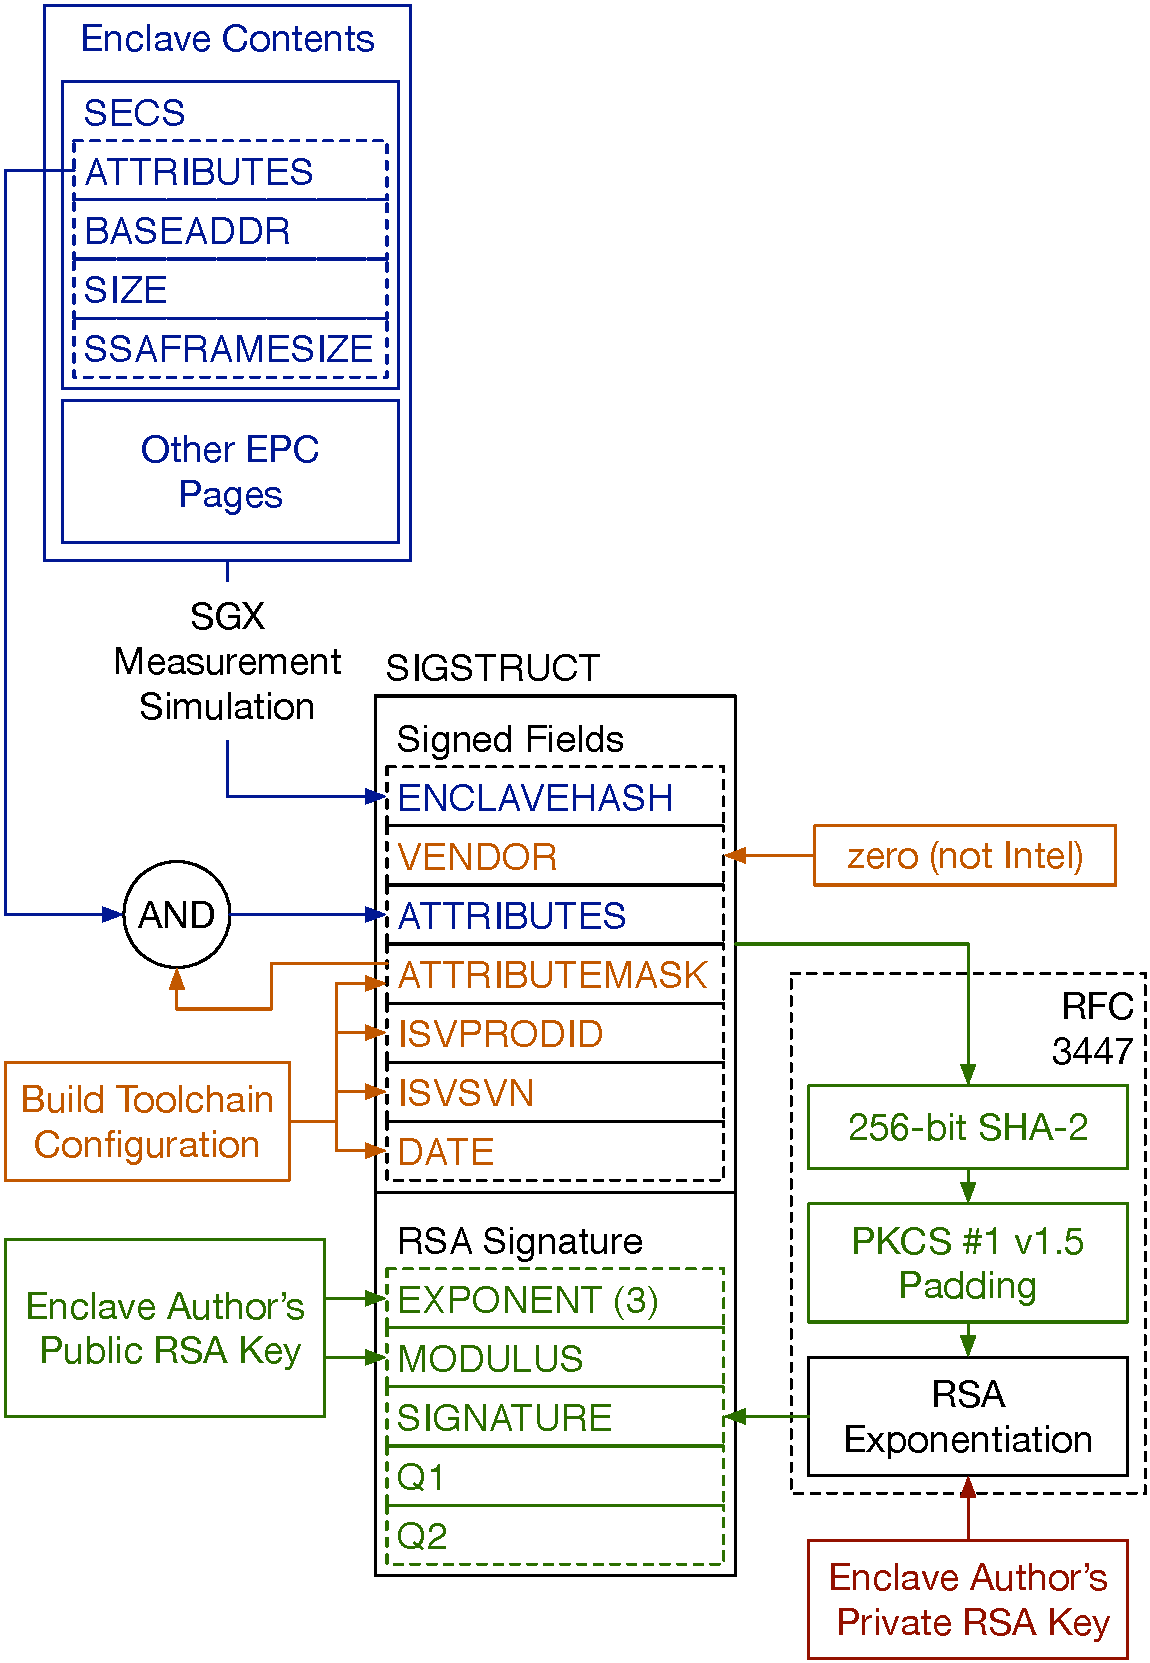
\includegraphics[width=85mm]{figures/sgx_sigstruct.pdf}
  \caption{
    An enclave's Signature Structure (SIGSTRUCT) is intended to be generated by
    an enclave building toolchain that has access to the enclave author's
    private RSA key.
  }
  \label{fig:sgx_sigstruct}
\end{figure}

A SIGSTRUCT certificate consists of metadata fields, the most interesting of
which are presented in Table~\ref{fig:sgx_sigstruct_info}, and an RSA
signature that guarantees the authenticity of the metadata, formatted as shown
in Table~\ref{fig:sgx_sigstruct_rsa}. The semantics of the fields will be
revealed in the following sections.

\begin{table}[hbt]
  \centering
  \begin{tabularx}{\columnwidth}{| l | r | X |}
  \hline
  \textbf{Field} & \textbf{Bytes} & \textbf{Description} \\
  \hline
  ENCLAVEHASH & 32 & Must equal the enclave's
                     measurement~(\S~\ref{sec:sgx_mrenclave}). \\
  \hline
  ISVPRODID & 32 & Differentiates modules signed by the same public key. \\
  \hline
  ISVSVN & 32 & Differentiates versions of the same module. \\
  \hline
  VENDOR & 4 & Differentiates Intel enclaves. \\
  \hline
  ATTRIBUTES & 16 & Constrains the enclave's attributes. \\
  \hline
  ATTRIBUTEMASK & 16 & Constrains the enclave's attributes. \\
  \hline
  \end{tabularx}
  \caption{
    A subset of the metadata fields in a SIGSTRUCT enclave certificate.
  }
  \label{fig:sgx_sigstruct_info}
\end{table}

\begin{table}[hbt]
  \centering
  \begin{tabularx}{\columnwidth}{| l | r | X |}
  \hline
  \textbf{Field} & \textbf{Bytes} & \textbf{Description} \\
  \hline
  MODULUS & 384 & RSA key modulus \\
  \hline
  EXPONENT & 4 & RSA key public exponent \\
  \hline
  SIGNATURE & 384 & RSA signature (See \S~\ref{sec:sgx_rsa_check}) \\
  \hline
  Q1 & 384 & Simplifies RSA signature verification.
             (See \S~\ref{sec:sgx_rsa_check}) \\
  \hline
  Q2 & 384 & Simplifies RSA signature verification.
             (See \S~\ref{sec:sgx_rsa_check}) \\
  \hline
  \end{tabularx}
  \caption{
    The format of the RSA signature used in a SIGSTRUCT enclave certificate.
  }
  \label{fig:sgx_sigstruct_rsa}
\end{table}

The enclave certificates must be signed by RSA
signatures~(\S~\ref{sec:integrity_crypto}) that follow the method described in
RFC 3447~\cite{jonsson2003pkcsv21}, using 256-bit SHA-2~\cite{fips2015shs} as
the hash function that reduces the input size, and the padding method described
in PKCS \#1 v1.5~\cite{kaliski1998pkcs1v15}.

The SGX implementation only supports 3072-bit RSA keys whose public exponent is
3. The key size is likely chosen to meet FIPS'
recommendation~\cite{fips2012keysize}, which makes SGX eligible for use in U.S.
government applications. The public exponent 3 affords a simplified signature
verification algorithm, which is described in \S~\ref{sec:sgx_rsa_check}. The
simplified algorithm also requires the fields Q1 and Q2 in the RSA signature,
which are also described in \S~\ref{sec:sgx_rsa_check}.


\subsubsection{Certificate-Based Enclave Identity}
\label{sec:sgx_certificate_identity}

An enclave's identity is determined by three fields in its
certificate~(\S~\ref{sec:sgx_sigstruct}): the modulus of the RSA key used to
sign the certificate (MODULUS), the enclave's product ID (ISVPRODID) and the
security version number (ISVSVN).

% EINIT: SDM S 41.3
% Enclave Signature Structure (SIGSTRUCT): SDM S 38.13

The public RSA key used to issue a certificate identifies the enclave's author.
All RSA keys used to issue enclave certificates must have the public exponent
set to 3, so they only have different moduli. Furthermore, SGX does not use
the entire modulus of a key, but rather a 256-bit SHA-2 hash of the modulus.
This is called a \textit{signer measurement} (MRSIGNER), to parallel the name
of \textit{enclave measurement} (MRENCLAVE) for the SHA-2 hash that identifies
an enclave's contents.

The SGX implementation relies on a hard-coded MRSIGNER value to recognize
certificates issued by Intel. Enclaves that have an Intel-issued certificate
can receive additional privileges, which are discussed in
\S~\ref{sec:sgx_attestation}.

An enclave author can use the same RSA key to issue certificates for enclaves
that represent different software modules. Each module is identified by a
unique Product ID (ISVPRODID) value. Conversely, all the enclaves whose
certificates have the same ISVPRODID and are issued by the same RSA key
(and therefore have the same MRENCLAVE) are assumed to represent different
versions of the same software module. Enclaves created by different authors are
always assumed to contain different software modules.

% Security Version Numbers: SDM S 39.4.2

Enclaves that represent different versions of a module can have different
security version numbers (SVN). The SGX design disallows the migration of
secrets from an enclave with a higher SVN to an enclave with a lower SVN. This
restriction is intended to assist with the distribution of security patches,
as follows.

If a security vulnerability is discovered in an enclave, the author can release
a fixed version with a higher SVN. As users upgrade, SGX will facilitate the
migration of secrets from the vulnerable version of the enclave to the fixed
version. Once an user's secrets are migrated, the SVN restrictions in SGX will
deflect any attack based on building the vulnerable enclave version and using
it to read the migrated secrets.

Software upgrades that add functionality should not be accompanied by an SVN
increase, as SGX allows secrets to be migrated freely between enclaves with
matching SVN values. As explained above, a software module's SVN should only be
incremented when a security vulnerability is found. SIGSTRUCT only allocates
2 bytes to the ISVSVN field, which translates to 65,536 possible SVN values.
This space can be exhausted if a large team (incorrectly) sets up a continunous
build system to allocate a new SVN for every software build that it produces,
and each code change triggers a build.


\subsubsection{CPU Security Version Numbers}
\label{sec:sgx_cpusvn}

% Security Version Numbers: SDM S 39.4.2
% Hardware Security Version: SDM S 39.4.2.2

The SGX implementation itself has a security version number (CPUSVN), which is
used in the key derivation process implemented~\cite{intel2013patent1} by
\texttt{EGETKEY}, in addition to the enclave's identity information. CPUSVN is
a 128-bit value that, according to the SDM, reflects the processor's microcode
update version.

% EINIT: SDM S 41.3

The SDM does not describe the structure of CPUSVN, but it states that comparing
CPUSVN values using integer comparison is not meaningful, and that only some
CPUSVN values are valid. Furthermore, CPUSVNs admit an ordering relationship
with has the same semantics as the ordering relationship between enclave SVNs.
Specifically, an SGX implementation will consider all SGX implementations with
lower SVNs to be compromised due to security vulnerabilities, and will not
trust them.

An SGX patent~\cite{intel2013patent1} discloses that CPUSVN is a concatenation
of small integers that represent the SVNs of the various components that make
up SGX's implementation. This representation is consistent with all the
statements made in the SDM.


\subsubsection{Establishing an Enclave's Identity}
\label{sec:sgx_einit_sigstruct}

When the \texttt{EINIT}~(\S~\ref{sec:sgx_einit_overview}) instruction prepares
an enclave for code execution, it also sets the SECS~(\S~\ref{sec:sgx_secs})
fields that make up the enclave's certificate-based identity, as shown in
Figure~\ref{fig:sgx_einit_sigstruct}.

\begin{figure}[hbt]
  \centering
  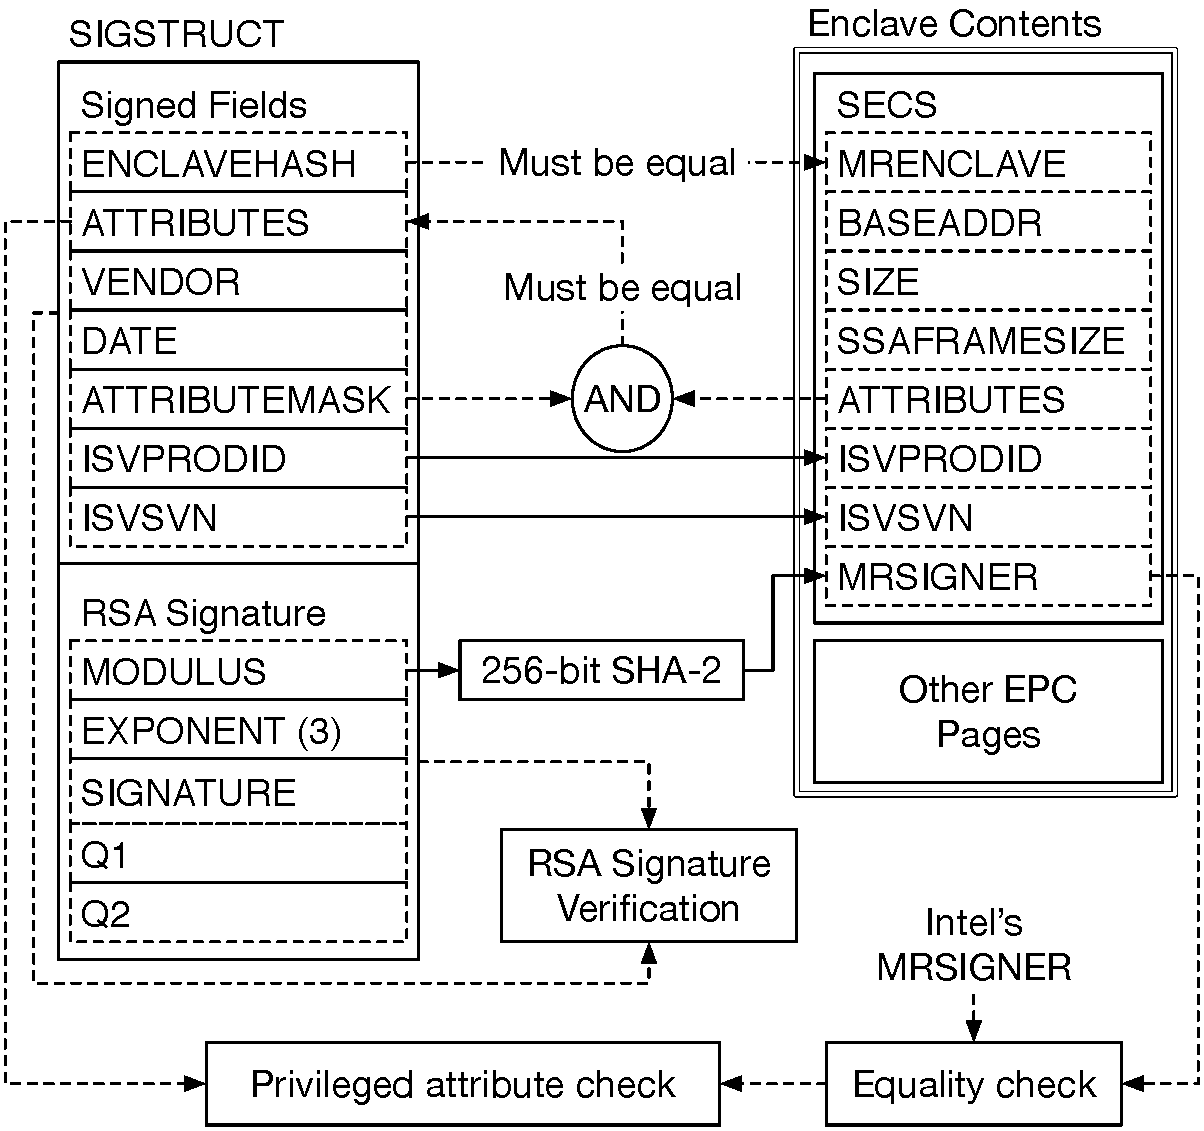
\includegraphics[width=85mm]{figures/sgx_einit_sigstruct.pdf}
  \caption{
    \texttt{EINIT} verifies the RSA signature in the enclave's certificate. If
    the certificate is valid, the information in it is used to populate the
    SECS fields that make up the enclave's certificate-based identity.
  }
  \label{fig:sgx_einit_sigstruct}
\end{figure}

% EINIT: SDM S 41.3
% Enclave Signature Structure (SIGSTRUCT): SDM S 38.13

Before using the information in the certificate, \texttt{EINIT} first verifies
its RSA signature. The SIGSTRUCT fields Q1 and Q2, along with the RSA exponent
3, facilitate a simplified verification algorithm, which is discussed in
\S~\ref{sec:sgx_rsa_check}.

If the SIGSTRUCT certificate is found to be properly signed, \texttt{EINIT}
follows the steps discussed in the following few paragraphs to ensure that the
certificate matches the enclave that is being initialized. Once the checks are
completed, \texttt{EINIT} computes MRSIGNER, the 256-bit SHA-2 hash of the
MODULUS field in the SIGSTRUCT, and writes it into the enclave's SECS.
\texttt{EINIT} also copies the ISVPRODID and ISVSVN fields from SIGSTRUCT into
the enclave's SECS. As explained in \S~\ref{sec:sgx_certificate_identity},
these fields make up the enclave's certificate-based identity.

\texttt{EINIT} performs a few checks to make sure that the enclave undergoing
initialization was indeed authorized by provided the SIGSTRUCT certificate. The
most obvious check involves making sure that the MRENCLAVE value in SIGSTRUCT
equals the enclave's measurement, which is stored in the MRENCLAVE field in
the enclave's SECS.

% SECS.ATTRIBUTES.XFRM: SDM S 42.7.2.1

However, MRENCLAVE does not cover the enclave's attributes, which are stored in
the ATTRIBUTES field of the SECS. As discussed in
\S~\ref{sec:sgx_ecreate_mrenclave_no_attributes}, omitting ATTRIBUTES from
MRENCLAVE facilitates writing enclaves that have optimized implementations
which can use architectural extensions when present, and also have fallback
implementations that work on CPUs without the extensions. Such enclaves can
execute corectly when built with a variety of values in the
XFRM~(\S~\ref{sec:sgx_secs_attributes}, \S~\ref{sec:sgx_ssa}) attribute. At
the same time, allowing system software to use arbitrary values in the
ATTRIBUTES field would compromise SGX's security guarantees.

When an enclave uses software
attestation~(\S~\ref{sec:generic_software_attestation}) to gain access to
secrets, the ATTRIBUTES value used to build it is included in the SGX
attestation signature~(\S~\ref{sec:sgx_attestation}). This gives the remote
party in the attestation process the opportunity to reject an enclave built
with an undesirable ATTRIBUTES value. However, when secrets are obtained using
the migration process facilitated by certificate-based identities, there is no
remote party that can check the enclave's attributes.

The SGX design solves this problem having enclave authors convey the set of
acceptable attribute values for an enclave in the ATTRIBUTES and ATTRIBUTEMASK
fields of the SIGSTRUCT certificate issued for the enclave. \texttt{EINIT} will
refuse to initialize an enclave using a SIGSTRUCT if the bitwise AND betwee
the ATTRIBUTES field in the enclave's SECS and the ATTRIBUTESMASK field in the
SIGSTRUCT does not equal the SIGSTRUCT's ATTRIBUTES field. This check prevents
enclaves with undesirable attributes from obtaining secrets using the migration
process that employs certificate-based identities.

Any enclave author can use SIGSTRUCT to request that specific bits in an
enclave's ATTRIBUTES field are cleared. However, certain bits can only be set
for enclaves that are signed by Intel. \texttt{EINIT} has a mask of restricted
ATTRIBUTES bits, discussed in \S~\ref{sec:sgx_attestation}. The \texttt{EINIT}
implementation contains a hard-coded MRSIGNER value that is used to identify
Intel's privileged enclaves, and only allows privileged enclaves to be built
with an ATTRIBUTES value that matches any of the bits in the restricted mask.
This check is essential to the security of the SGX software attestation
process, which is described in \S~\ref{sec:sgx_attestation}.

Last, \texttt{EINIT} also inspects the VENDOR field in SIGSTRUCT. The SDM
description of the VENDOR field in the section dedicated to SIGSTRUCT suggests
that the field is essentially used to distinguish between special enclaves
signed by Intel, which use a VENDOR value of 0x8086, and everyone else's
enclaves, which should use a VENDOR value of zero. However, the \textit{EINIT}
pseudocode seems to imply that the SGX implementation only checks that
VENDOR is either zero or 0x8086.


\subsubsection{Enclave Key Derivation}
\label{sec:sgx_egetkey}

SGX's secret migration mechanism is based on the symmetric key derivation
service that is offered to enclaves by the \texttt{EGETKEY} instruction,
illustrated in Figure~\ref{fig:sgx_egetkey}.

\begin{figure}[hbt]
  \centering
  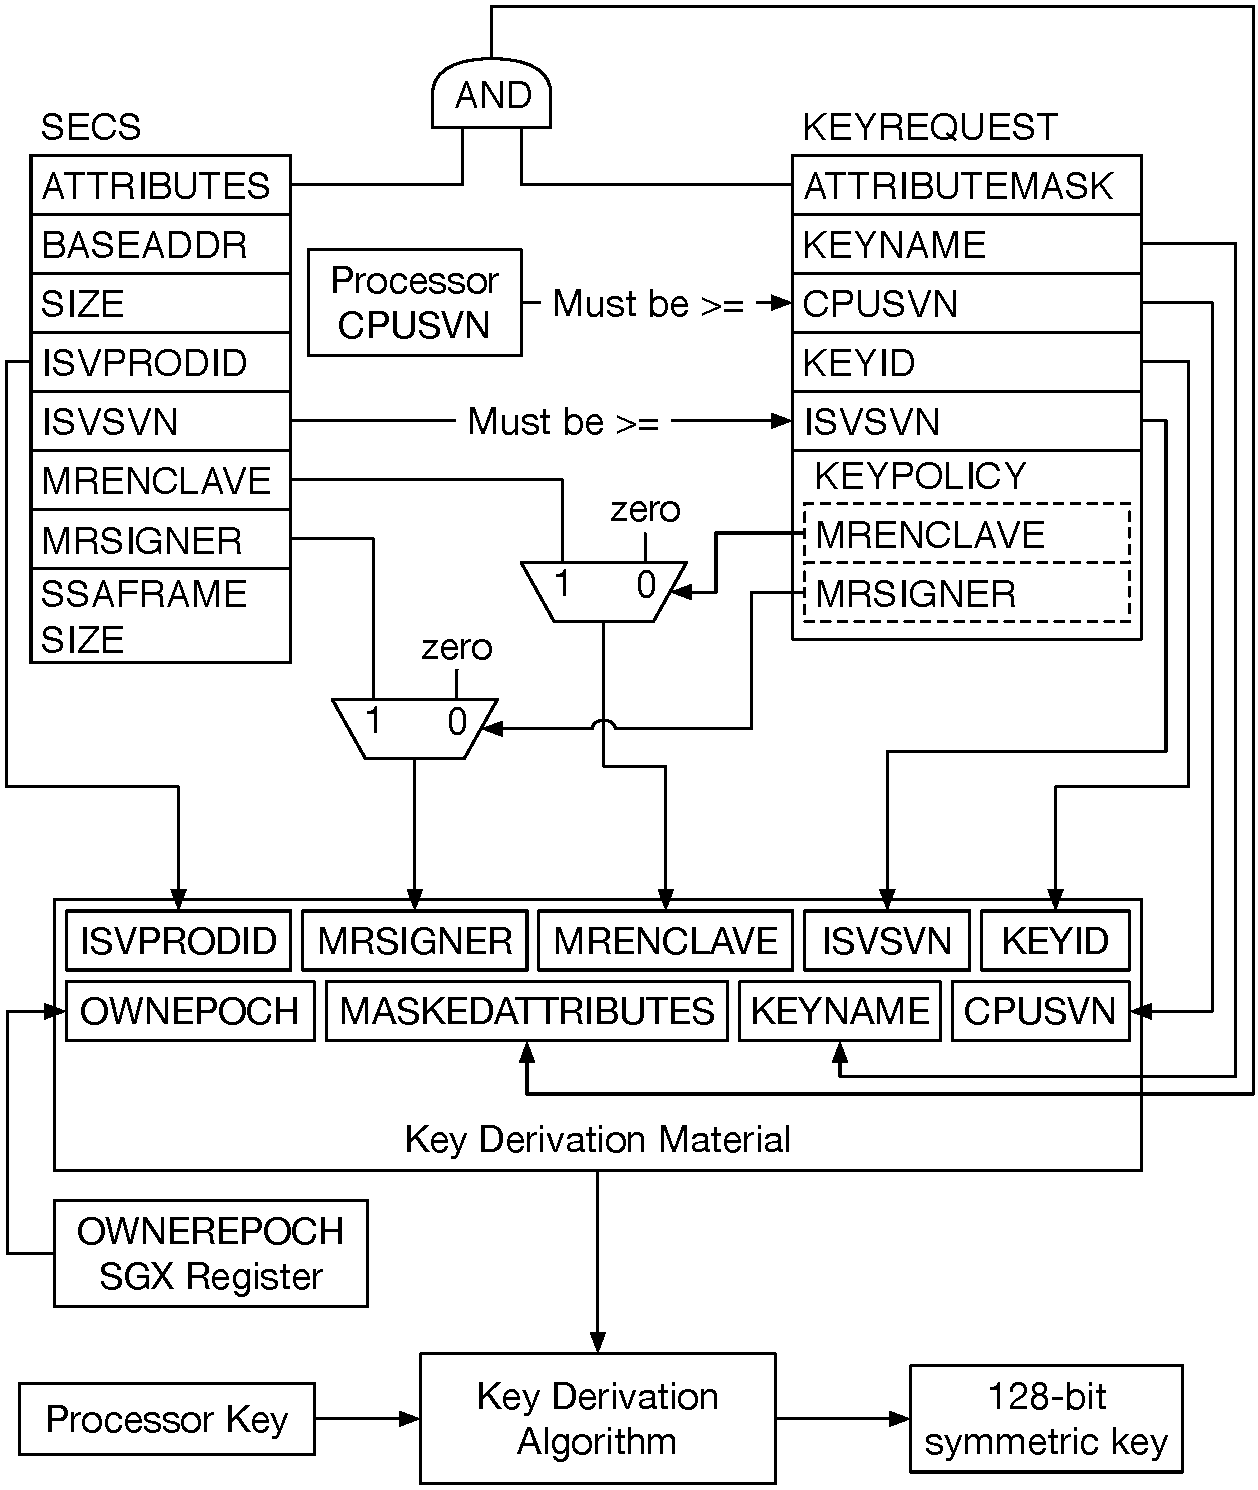
\includegraphics[width=87mm]{figures/sgx_egetkey.pdf}
  \caption{
    \texttt{EGETKEY} implements a key derivation service that is primarily used
    by SGX's secret migration feature. The key derivation material is derived
    from the SECS of the calling enclave, the information in a Key Request
    structure, and a.
  }
  \label{fig:sgx_egetkey}
\end{figure}

The keys produced by \texttt{EGETKEY} are derived based on the identity
information in the current enclave's SECS and on a secret stored in secure
hardware inside the SGX-enabled processor. The pieces of information used to
derive the keys are selected by a Key Request (KEYREQUEST) structure, shown in
Table~\ref{fig:sgx_keyrequest}.

% Key Request (KEYREQUEST): SDM S 38.17

\begin{table}[hbt]
  \centering
  \begin{tabularx}{\columnwidth}{| l | r | X |}
  \hline
  \textbf{Field} & \textbf{Bytes} & \textbf{Description} \\
  \hline
  KEYNAME & 2 & The desired key type; secret migration uses ``Seal'' keys \\
  \hline
  KEYPOLICY & 2 & The identity information (MRENCLAVE and/or MRSIGNER) \\
  \hline
  ISVSVN & 2 & The enclave SVN used in derivation\\
  \hline
  CPUSVN & 16 & SGX implementation SVN used in derivation \\
  \hline
  ATTRIBUTEMASK & 16 & Selects enclave attributes \\
  \hline
  KEYID & 32 & Random bytes \\
  \hline
  \end{tabularx}
  \caption{
    A subset of the fields in the KEYREQUEST structure. These fields
  }
  \label{fig:sgx_keyrequest}
\end{table}

% KDF uses FIPS SP 800-180 and AES-CMAC
%   US 8,972,746 B2 - 44:17-29
%   US 9,807,200 B2 - 42:32-48
% EGETKEY uses a fused key and derivation
%   US 8,972,746 B2 - 51:34-65
%   US 9,807,200 B2 - 49:34-65
%   ISCA SGX Slide 99

The SDM does not specify the key derivation algorithm, but the SGX
patents~\cite{intel2013patent1, intel2013patent2} disclose that the keys are
derived using the method described in FIPS SP 800-108~\cite{fips2009kdf} using
AES-CMAC~\cite{fips2005cmac} as a Pseudo-Random Function (PRF). The same
patents state that the secret used for key derivation is stored in e-fuses in
the CPU, which is confirmed by the ISCA 2015 SGX
tutorial~\cite{intel2015iscasgx}.

This additional information implies that all \texttt{EGETKEY} invocations that
use the same key derivation material will result in the same key, even across
CPU power cycles. Furthermore, it is impossible for an adversary to obtain the
key produced from a specific key derivation material without access to the
secret stored in the CPU's e-fuses. The following paragraphs discuss the pieces
of data used in the key derivation material.

% Key Request (KEYREQUEST): SDM S 38.17
% EGETKEY: SDM S 41.4.1
% Key Derivation: SDM Table 41-43

The KEYNAME field in KEYREQUEST always participates in the key generation
material. It indicates the type of the key to be generated. While the SGX
design define a few key types, the secret migration feature always uses ``Seal
keys''. The other key types are used by the SGX software attestation process,
which will be outlined in \S~\ref{sec:sgx_attestation}.

The KEYPOLICY field in KEYREQUEST has two flags that indicate if the MRENCLAVE
and MRSIGNER fields in the enclave's SECS will be used for key derivation.
Although the fields admits 4 values, only two seem to make sense, as argued
below.

Setting the MRENCLAVE flag in KEYPOLICY ties the derived key to the current
enclave's measurement, which reflects its contents. No other enclave will be
able to obtain the same key. This is useful when the derived key is used to
encrypt enclave secrets so they can be stored by system software in
non-volatile memory, and thus survive power cycles.

If the MRSIGNER flag in KEYPOLICY is set, the derived key is tied to the public
RSA key that issued the enclave's certificate. Therefore, other enclaves issued
by the same author may be able to obtain the same key, subject to the
restrictions below. This is the only KEYPOLICY value that allows for secret
migration.

It makes little sense to have no flag set in KEYPOLICY. In this case, the
derived key has no useful security property, as it can be obtained by other
enclaves that are completely unrelated to the enclave invoking
\texttt{EGETKEY}. Conversely, setting both flags is redundant, as setting
MRENCLAVE alone will cause the derived key to be tied to the current enclave,
which is the strictest possible policy.

The KEYREQUEST structure specifies the enclave
SVN~(ISVSVN,~\S~\ref{sec:sgx_certificate_identity}) and SGX implementation
SVN~(CPUSVN,~\S~\ref{sec:sgx_cpusvn}) that will be used in the key derivation
process. However, \texttt{EGETKEY} will reject the derivation request and
produce an error code if the desired enclave SVN is greater than the current
enclave's SVN, or if the desired SGX implementation SVN is greater than the
current implementation's SVN.

The SVN restrictions prevent the migration of secrets from enclaves with higher
SVNs to enclaves with lower SVNs, or from SGX implementations with higher SVNs
to implementations with lower SVNs. \S~\ref{sec:sgx_certificate_identity}
argues that the SVN restrictions can reduce the impact of security
vulnerabilities in enclaves and in SGX's implementation.

\texttt{EGETKEY} always uses the ISVPROD value from the current enclave's SECS
for key derivation. It follows that secrets can never flow between enclaves
whose SIGSTRUCT certificates assign them different Product IDs.

Similarly, the key derivation material always includes the value of an 128-bit
Owner Epoch (OWNEREPOCH) SGX configuration register. This register is intended
to be set by the computer's firmware to a value that represents the computer's
current user. If the computer changes ownership, the new owner can change the
Owner Epoch value, which invalidates all the old keys produced by
\texttt{EGETKEY}.

The \texttt{EGETKEY} derivation material also includes a 256-bit value supplied
by the enclave, in the KEYID field. This makes it possible for an enclave to
generate a collection of keys from \texttt{EGETKEY}, instead of a single key.
The SDM states that KEYID should be populated with a random number, and is
intended to help prevent key wear-out.

Last, the key derivation material includes the bitwise AND of the
ATTRIBUTES~(\S~\ref{sec:sgx_secs_attributes}) field in the enclave's SECS and
the ATTRIBUTESMASK field in the KEYREQUEST structure. The mask has the effect
of removing some of the ATTRIBUTES bits from the key derivation material,
making it possible to migrate secrets between enclaves with different
attributes. \S~\ref{sec:sgx_ecreate_mrenclave_no_attributes} and
\S~\ref{sec:sgx_einit_sigstruct} explain the need for this feature, as well as
its security implications.

Before adding the masked attributes value to the key generation material, the
\texttt{EGETKEY} implementation forces the mask bits corresponding to the
INIT and DEBUG attributes~(\S~\ref{sec:sgx_secs_attributes}) to be set. From a
practical standpoint, this means that secrets will never be migrated between
enclaves that support debugging and production enclaves.
